\section{Deskriptive  Analyse}\label{descriptiv}

Tabelle \ref{varbeschreibung} enthält eine Übersicht mit den erzeugten Variablen. Diese werden in diesem Kapitel näher betrachtet. Als Position wird im folgenden die Nummer eines Kontaktpunktes innerhalb eines Funnels bezeichnet. Das heißt für jeden Funnel nimmt der erste Kontakt die Position $1$ an. Alle folgenden Abbildungen dieses Berichts wurden mit dem R-Paket \textit{ggplot2} \cite{ggplot2} erzeugt.
\begin{table}[H]
    \begin{center}
\begin{tabular}{|c|p{10cm}|}
		\hline $ clickCount \in \mathbb{N} $ & Anzahl an \textit{Clicks} bis zur aktuellen Position\\
    \hline $ hasClicked\in\{0,1\} $  & Dummyvariable, die angibt ob vor der aktuellen Position schon geklicked wurde ($1$) oder nicht ($0$). \\
		\hline $ campaign $ & Kampagne der aktuellen Position\\ 
    \hline $ campaignLast $ & Kampagne der vorherigen Position\\ 
    \hline $ campaignLast2 $  & Kampagne der vorletzten Position\\
    \hline $ weekday \in \{Montag,...\}$ & Wochentag des Kontaktes  \\
    \hline $ hour \in \{0,1,\dots, 23\} $  & Uhrzeit des Kontaktes \\
    \hline $ timeSinceLast \in \mathbb{R}$  & Zeitdifferenz zwischen aktueller und vorheriger Position\\
    \hline $ timeSinceFirst \in \mathbb{R} $ & Zeitdifferenz zwischen aktueller und erster Position\\
    \hline$ freq \in \mathbb{R} $ & Frequenz der Kontaktpunkte in einem Funnel\\
    \hline
\end{tabular} 
 \end{center}
 \caption{Variablenbeschreibung}\label{varbeschreibung}
\end{table}

\subsection{Views in den konvertierten Funnels}\label{plotsViews}

\subsubsection*{clickCount}
Aufgrund der in Kapitel \ref{datenlage} beschriebenen Problematik bei der Datenerhebung der \textit{Views} können die Variablen \textit{clickCount} und \textit{hasClicked} nur in den konvertierten Funnels betrachtet werden. In Abbildung \ref{clickCount} ist der \textit{clickCount} dargestellt. Auf der $x$-Achse ist die Position aufgetragen und auf der $y$-Achse der \textit{clickCount}, das heißt die Häufigkeit der \textit{Clicks} gemittelt über alle konvertierten Funnels für jede Position. Die rote Diagonale wäre erreicht, wenn die konvertierten Funnels nur aus \textit{Clicks} bestehen würden. Es ist zu erkennen, dass die Linie mit der Position ansteigt. An Position $100$ ist die mittlere Anzahl der Clicks 13.7, das heißt im Mittel bestehen die ersten $100$ Kontakte eines Funnels aus $14$ \textit{Clicks} und $86$ \textit{Views}. Die Anzahl der \textit{Views} übersteigt die Anzahl der \textit{Clicks} also deutlich.\\
\begin{figure}[H]
    \centering
    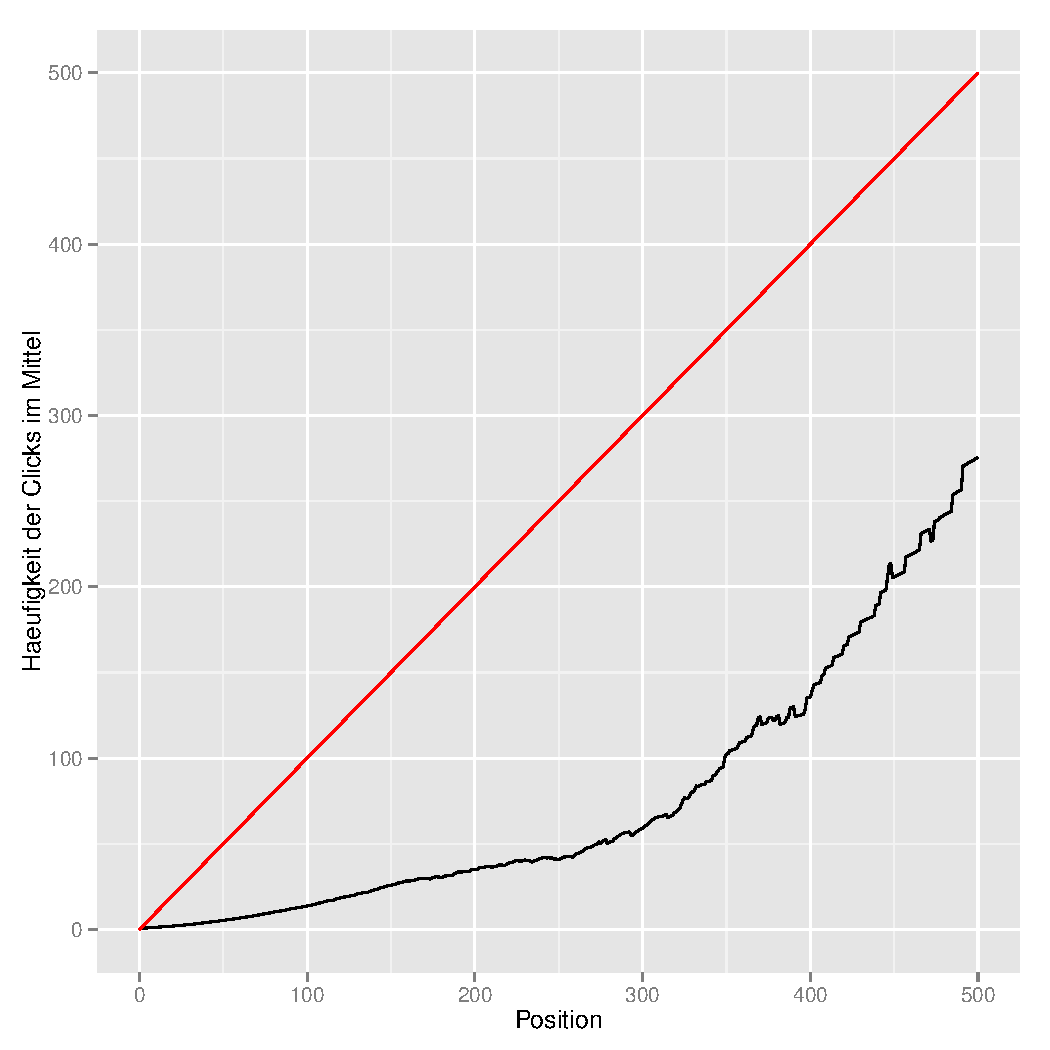
\includegraphics[scale=0.3]{clickCountSucc.pdf}
    \caption[Häufigkeit der Clicks im Mittel]{Häufigkeit der Clicks im Mittel für jede Position}
    \label{clickCount}
\end{figure}

\subsubsection*{hasClicked}
Die Variable \textit{hasClicked} (siehe Abbildung \ref{hasClicked}) gibt für jede Position den Anteil der Funnels an, die bis dorthin mindestens einen \textit{Click} enthalten. Dieser Wert nimmt zwischen Position $1$ und Position $7$ ab. Dies ist dadurch zu erklären, dass es viele Funnels gibt, die \textit{Clicks} enthalten und deren Länge kleiner als $6$ ist. Sobald diese Funnels beendet sind, werden sie an der nächsten Position selbstverständlich nicht mehr berücksichtigt. Ab Position $7$ steigt die Kurve dann bis zur $1$ an. Ein Wert von $1$ bedeutet, dass alle Funnels bereits einen \textit{Click} hatten.
\begin{figure}[H]
    \centering
    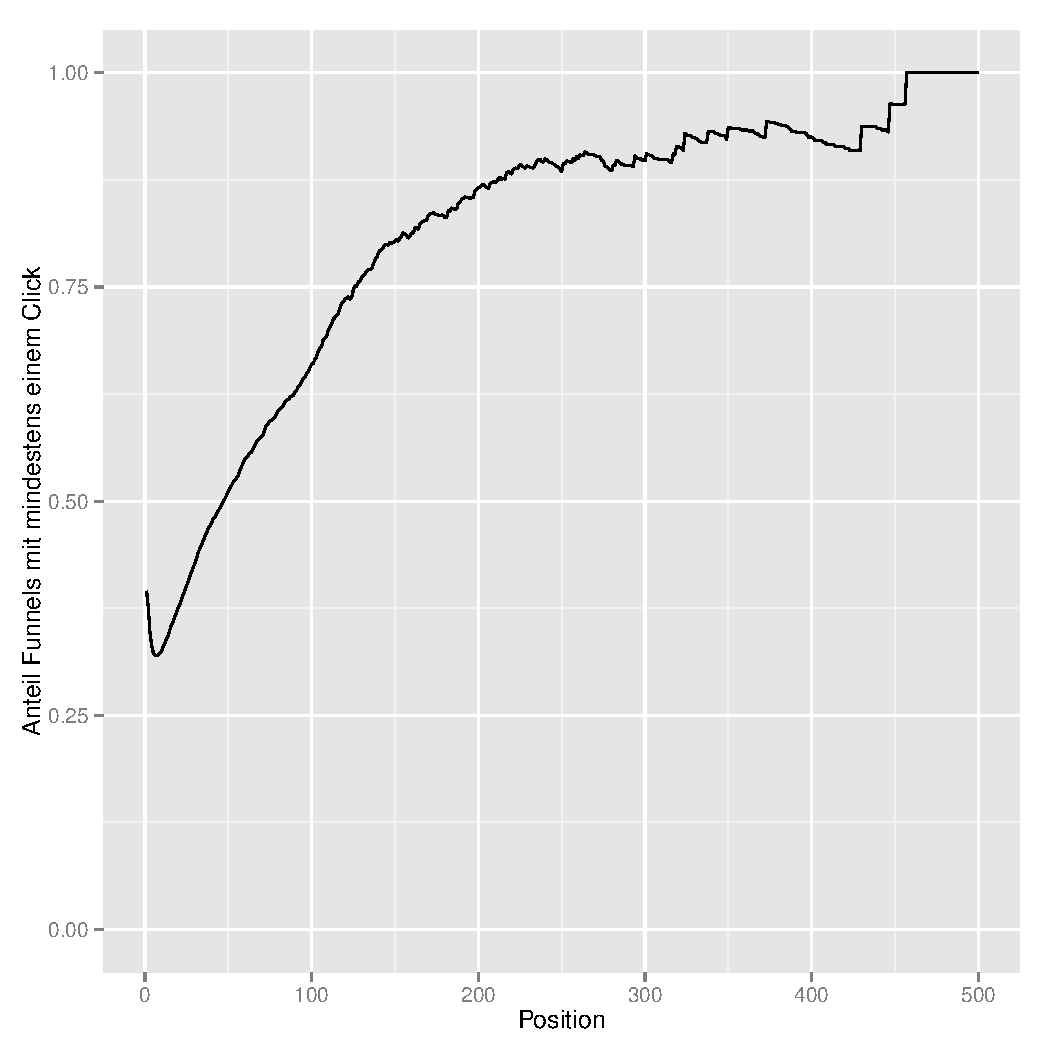
\includegraphics[scale=0.3]{hasClickedSucc.pdf}
    \caption[Anteil Funnels mit mindestens einem Click]{Anteil der Funnels mit mindestems einem Click für jede Position}
    \label{hasClicked}
\end{figure}

\subsubsection*{campaign}
In Kapitel \ref{datenlage} wurde bereits eine Übersicht über die Kampagnen gegeben. Abbildung \ref{campaignSucc} enthält die Verteilung dieser $17$ Kategorien in den konvertierten Funnels, das heißt auf der $x$-Achse ist die relative Häufigkeit aufgetragen und auf der $y$-Achse die Kategorien. Die orangefarbigen Balken repräsentieren die Verteilung in den konvertierten Funnels nur mit \textit{Clicks}, wie sie auch in den späteren Analysen verwendet werden. Die blauen Balken enthalten \textit{Clicks} und \textit{Views}.\\
Es ist zu erkennen, dass die Kampagne \textit{Display} bei den Funnels mit \textit{Views} $84 \%$ der gesamten Kontaktpunkte ausmacht. Das heißt die Bannerschaltungen überwiegen deutlich und ansonsten hat nur \textit{Direct} einen Anteil von über $5 \%$.\\
Werden die \textit{Views} nicht berücksichtigt so verteilen sich die Kampagnen besser. \textit{Display} macht jetzt weniger als $10 \%$ aus und \textit{Direct} ist mit über $35 \%$ die am häufigsten auftretende Kampagne. Außerdem haben auch \textit{SEO}, \textit{SEM - Generisch}, \textit{SEM - Brand}, \textit{Kooperationen - Immoscout24} und \textit{Affiliate - Partnerprogramm} einen Anteil von über $5 \%$. Die restlichen Kampagnen, besonders \textit{Social Media}, machen nur einen kleinen Teil der Daten aus.
\begin{figure}[H]
    \centering
    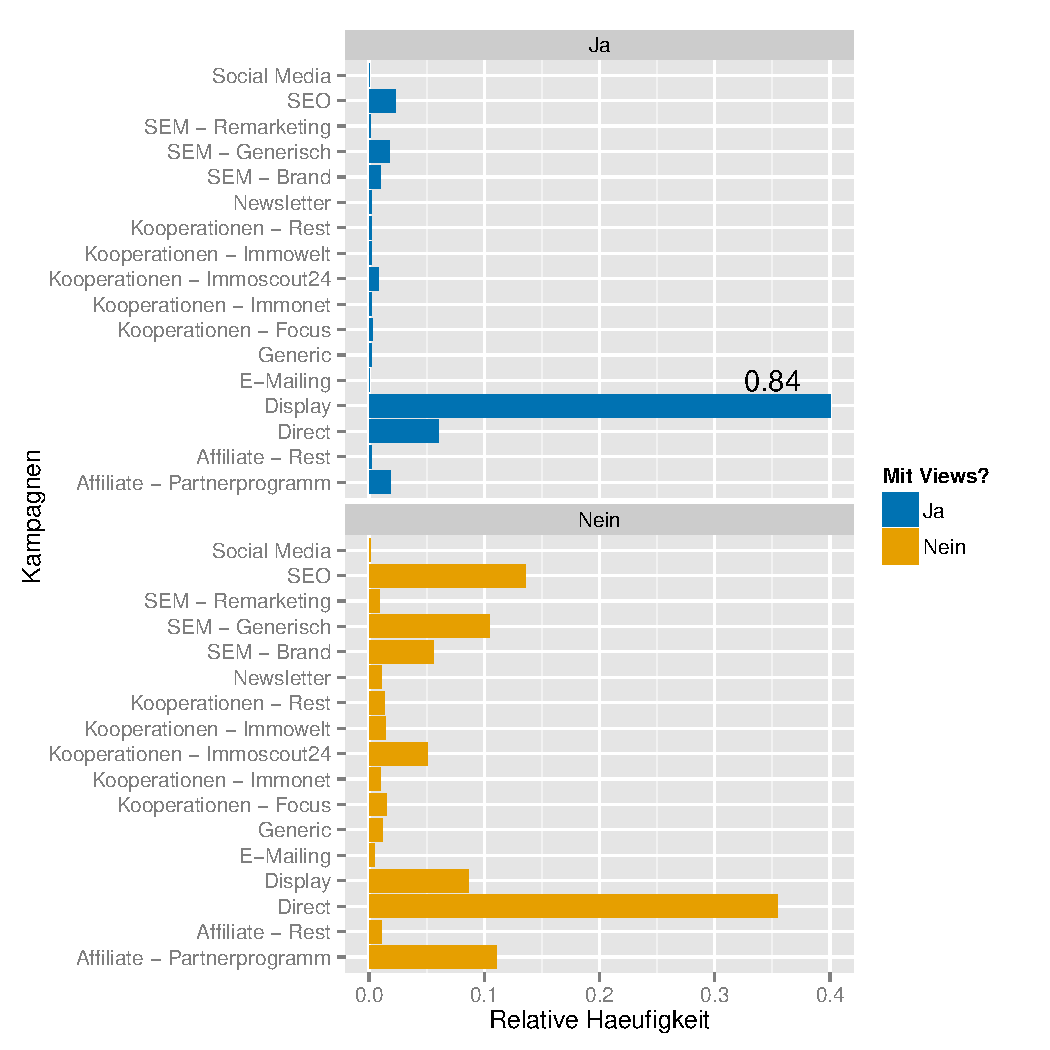
\includegraphics[scale=0.5]{campaignSucc.pdf}
    \caption[Kampagnen der konvertierten Funnels]{Kampagnen der konvertierten Funnels mit und ohne Views}
    \label{campaignSucc}
\end{figure}

\subsection{Vergleich von konvertierten und nicht-konvertierten Funnels}

Nachdem bis hierhin nur die konvertierten Funnels mit Augenmerk auf den \textit{Views} betrachtet wurden, sollen in diesem Kapitel die konvertierten und nicht-konvertierten Funnels miteinander verglichen werden. Das heißt, die \textit{Views} werden von nun an nicht mehr in die Analysen mit einbezogen.

\subsubsection*{weekday}
Die Variable \textit{Weekday} gibt an, an welchem Wochentag ein Konaktpunkt aufgetreten ist. Abbildung \ref{weekday} enthält diesbezüglich Histogramme. Die orangefarbigen Balken entsprechen den konvertierten und die blauen Balken den nicht-konvertierten Funnels. Für weitere Plots in diesem Kapitel gelten die selben Farben. Außerdem ergeben die blauen und orangefarbigen Balken erneut aufsummiert jeweils eins, das heißt sie spiegeln die Verteilung wieder.\\
Es ist zu erkennen, dass die Häufigkeit der Kontaktpunkte von Montag bis Samstag sinkt. Dieser Trend ist in den konvertierten Funnels etwas stärker. Dort sinkt die relative Häufigkeit von $ 0.17 $ am Montag auf $ 0.09 $ am Samstag. Bei den nicht-konvertierten Funnels sinkt die relative Häufigkeit von $ 0.15 $ am Montag auf $ 0.11 $ am Samstag. Außerdem ist der Sonntag bei den nicht-konvertierten mit Abstand der stärkste Tag, während in den konvertierten Funnels der Montag etwas stärker ist als der Sonntag.
\begin{figure}[H]
    \centering
    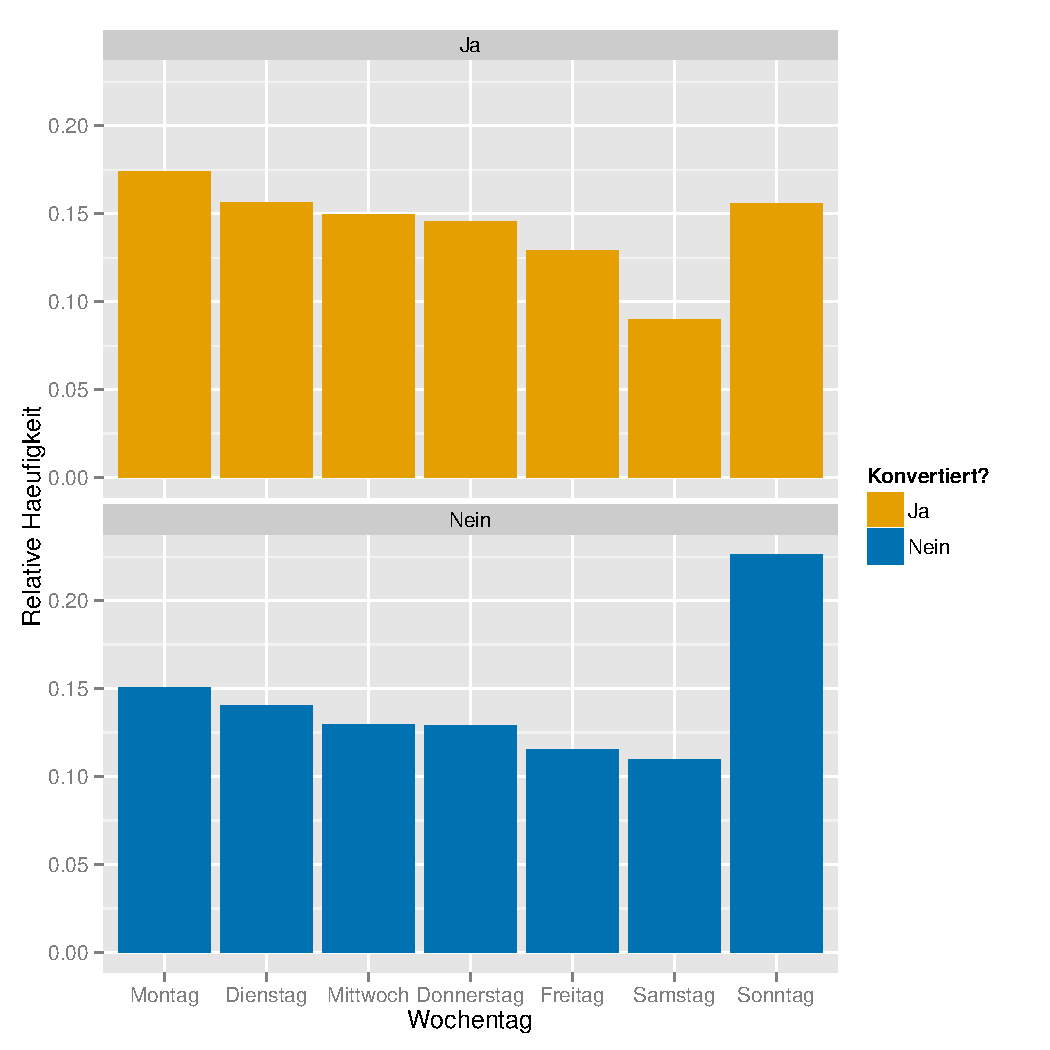
\includegraphics[scale=0.5]{weekday.pdf}
    \caption{Wochentage der Kontaktpunkte}
    \label{weekday}
\end{figure}

\subsubsection*{hour}
Analog zu der Abbildung mit den Wochentagen, enthält Abbildung \ref{hour} Informationen zu der Uhrzeit der Kontaktpunkte in konvertierten und nicht-konvertierten Funnels. Hierfür wurden die Minutenangaben der Uhrzeit jeweils abgeschnitten, so dass \textit{hour} nur die Werte $0,1,...,23$ annehmen kann.\\
Die Verteilungen in konvertierten und nicht-konvertierten Funnels sind sich sehr ähnlich, so dass keine deutlichen Unterschiede erkennbar sind. Insgesamt kann man zusammenfassen, dass in der Nacht zwischen zwei und sechs Uhr sehr wenige Kontaktpunkte stattfinden. Ab sechs Uhr steigt die relative Häufigkeit der Kontaktpunkte bis circa elf Uhr an und dann bleibt sie konstant bis circa $21$ Uhr. Daraufhin fällt die relative Häufigkeit wieder ab. Dies ist lediglich darauf zurück zu führen, dass nachts weniger Menschen online sind.
\begin{figure}[H]
    \centering
    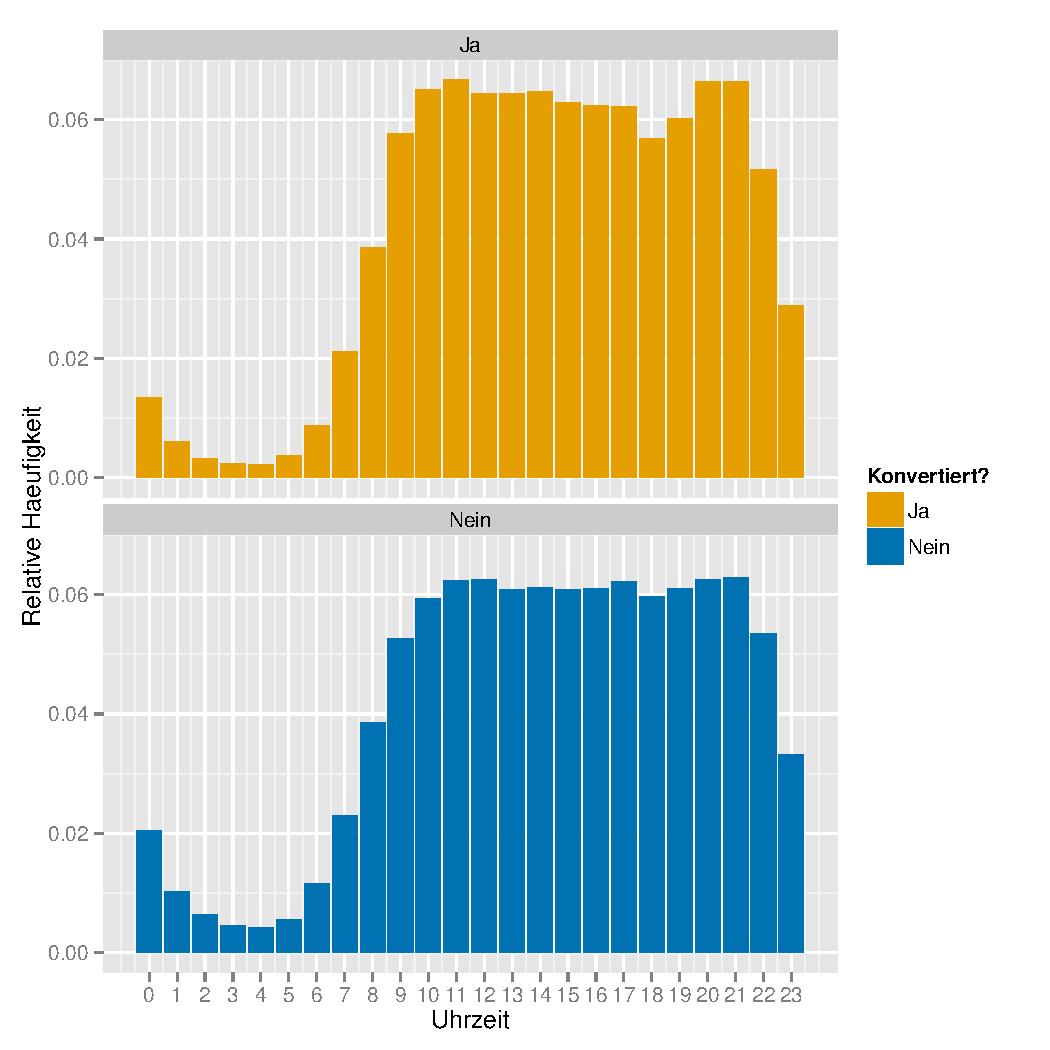
\includegraphics[scale=0.5]{hour.pdf}
    \caption{Uhrzeit der Kontaktpunkte}
    \label{hour}
\end{figure}

\subsubsection*{campaign}
Wie bereits in Kapitel \ref{plotsViews} werden die verschiedenen Kampagnen betrachtet. Allerdings werden an dieser Stelle die konvertierten und nicht-konvertierten Funnels miteinander verglichen, wobei die \textit{Views} nicht berücksichtigt werden (siehe Abbildung \ref{campaign}). Das heißt, die Verteilung der konvertierten Funnels ohne \textit{Views} aus Kapitel \ref{plotsViews} entspricht der Verteilung der konvertierten Funnels in diesem Abschnitt. Eine nähere Beschreibung der unterschiedlichen Kampagnen ist in Abbildung \ref{beschreibungCampaign} zu finden.\\
Die Verteilung in den konvertierten Funnels wurde bereits in Kapitel \ref{plotsViews} etwas näher beleuchtet. Während dort \textit{Direct} mit Abstand die stärkste Kampagne ist, sind in den nicht-konvertierten Funnels \textit{Affiliate - Partnerprogramm} und \textit{Display} die stärksten Kategorien und \textit{Direct} ist lediglich drittstärkste mit einer relativen Häufigkeit von $ 0.123 $. Wie in den konvertierten Funnels haben hier auch \textit{SEO}, \textit{SEM - Generisch} und \textit{Kooperationen - Immoscout24} einen Anteil von über $5 \%$. \textit{SEM - Brand} tritt in den konvertierten Funnels deutlich häufiger auf als in den nicht-konvertierten. Für die restlichen Kampagnen liegen insgesamt wenige Daten vor.

\begin{figure}[H]
	\centering
	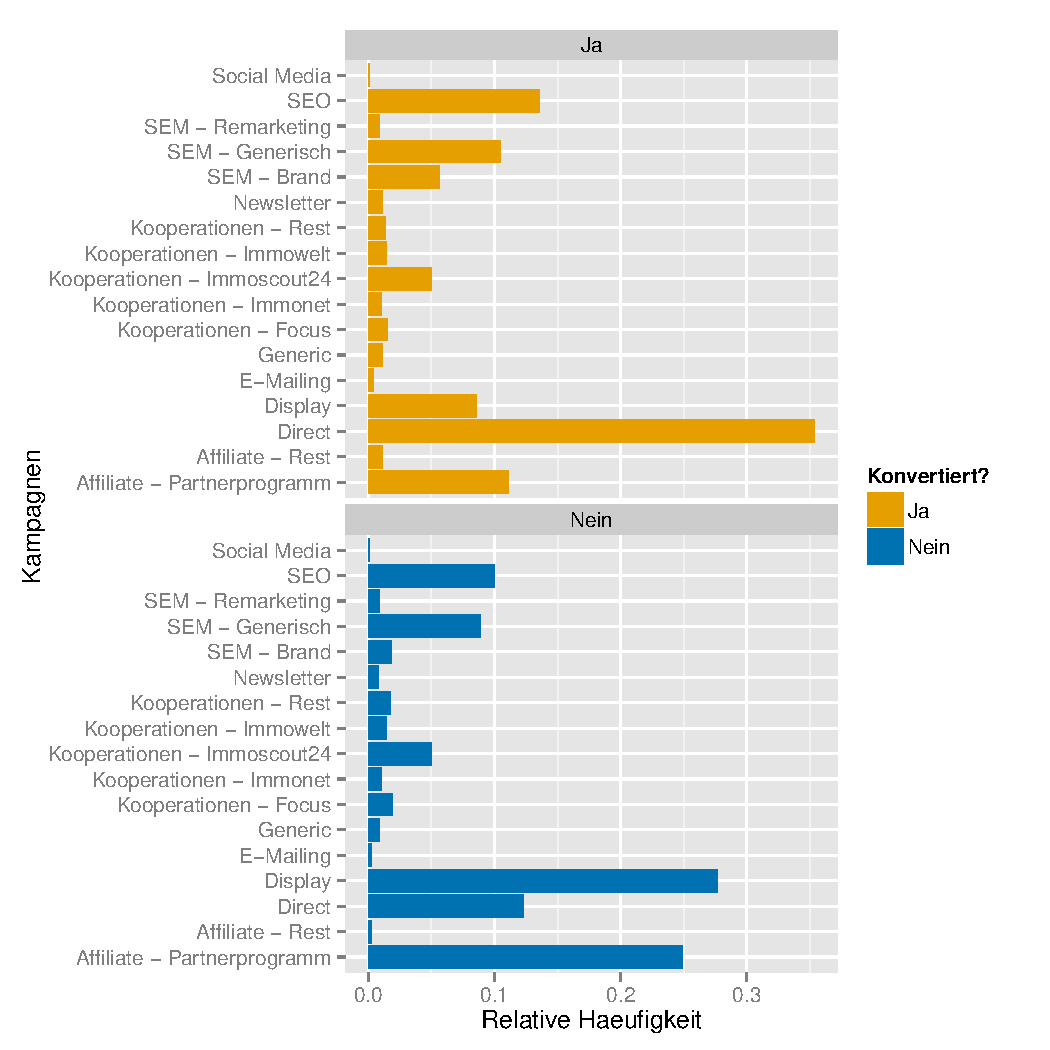
\includegraphics[scale=0.5]{campaign.pdf}
	\caption{Kampagnen der konvertierten und nicht-konvertierten Funnels}
	\label{campaign}
\end{figure}
    
\subsubsection*{funnelLength}
Die \textit{funnelLength} gibt die Anzahl der Kontaktpunkte eines Funnels an. In Abbildung \ref{funnelLength} sind nur diejenigen Funnels dargestellt, deren Länge $20$ Kontaktpunkte nicht überschreitet, da es, relativ gesehen, sehr wenige längere Funnels gibt.\\
Von den nicht-konvertierten Funnels haben $75 \%$ nur einen Kontaktpunkt. Von dort nimmt die relative Häufigkeit der Funnels mit steigender Länge sehr schnell ab. Von den konvertierten Funnels haben $41 \%$ nur einen Kontaktpunkt. Das heißt, relativ betrachtet, gibt es dort mehr Funnels mit mehreren Kontaktpunkten. Allerdings gibt es insgesamt deutlich mehr nicht-konvertierte als konvertierte Funnels, so dass die absoluten Anzahl für die nicht-konvertierten stets größer ist. Der Mittelwert beziehungsweise der Median der Länge der Funnels ist bei den konvertierten Funnels $4.1$ beziehungsweise $2$ und bei den nicht-konvertierten $1.66$ beziehungsweise $1$. 

\begin{figure}[H]
    \centering
    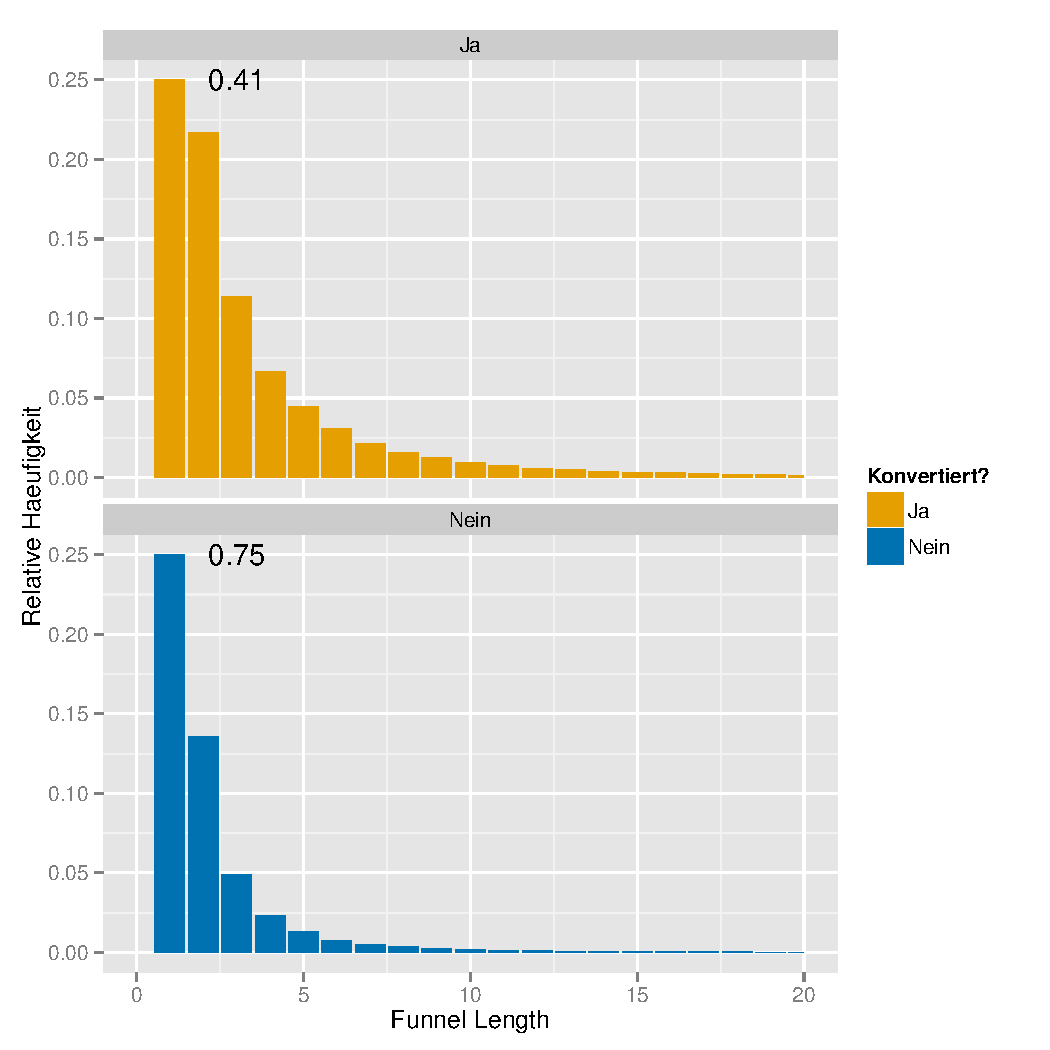
\includegraphics[scale=0.5]{funnelLength_First.pdf}
    \caption[Länge der Funnels]{Länge der Funnels in konvertierten und nicht-konvertierten Funnels}
    \label{funnelLength}
\end{figure}

\subsubsection*{timeSinceFirst}
Das Feature \textit{timeSinceFirst} gibt für jede Position die verstrichene Zeit seit dem ersten Kontaktpunkt an. In Abbildung \ref{timeSinceFirst} wird dieses nur für die letzte Position der Funnels geplottet, so dass die Gesamt-Beobachtungsdauer der Funnels betrachtet wird, das heißt die verstrichene Zeit zwischen dem ersten und dem letzten Kontaktpunkt eines jeden Funnels. Auf der $x$-Achse ist die Beobachtungsdauer in Tagen von $0$ bis $50$ aufgetragen.\\
Hier gestaltet sich ein ähnliches Bild wie in Abbildung \ref{funnelLength}. Allerdings muss berücksichtigt werden, dass die \textit{timeSinceFirst} für die erste Position nicht existiert und somit hier nicht berücksichtigt wird. Von den nicht-konvertierten Funnels haben $58 \%$ eine Beobachtungsdauer von weniger als einem Tag. Längere Beobachtungsdauern treten deutlich seltener auf. Von den konvertierten Funnels haben $33 \%$ eine Beobachtungsdauer von weniger als einem Tag und längere Beobachtungsdauern treten, relativ betrachtet, häufiger auf als in den nicht-konvertierten Funnels.\\
Auffällig sind außerdem die Hückel, die im Rhythmus von sieben Tagen auftreten. Dies ist darauf zurückzuführen, dass Sonntag und Montag die zwei Tage mit den häufigsten Kontakten sind und beispielsweise Bannerschaltungen am Wochenende besonders häufig eingesetzt werden. Bei den konvertierten Funnels liegt der Mittelwert der Beobachtungsdauer bei $21.1$ Tagen und bei den nicht-konvertierten Funnels bei $5.3$ Tagen. 
\begin{figure}[H]
    \centering
    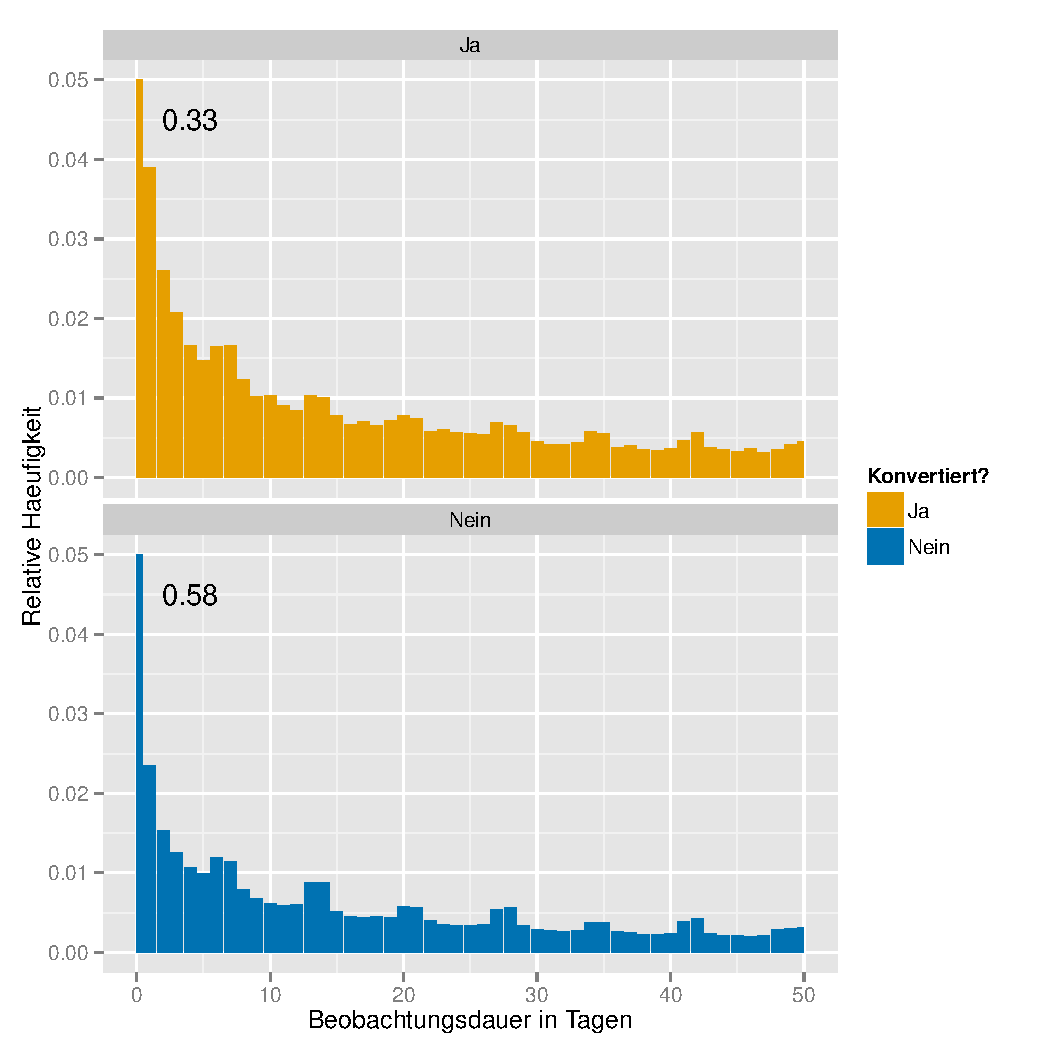
\includegraphics[scale=0.5]{timeSinceFirst_Last.pdf}
    \caption[Beobachtungsdauer in Tagen]{Beobachtungsdauer in Tagen der konvertierten und nicht-konvertierten Funnels}
    \label{timeSinceFirst}
\end{figure}

\subsubsection*{timeSinceLast}
Die Variable \textit{timeSinceLast} gibt die verstrichene Zeit zwischen zwei aufeinander folgenden Kontaktpunkte an. Diese ist in Abbildung \ref{timeSinceLast} abgebildet, wobei nun alle Kontaktpunkte berücksichtigt werden und nicht nur der letzte, wie es bei \textit{timeSinceFirst} der Fall war.\\
Die relative Häufigkeit der Abstände, die kürzer als ein Tag sind ist bei den nicht-konvertierten Funnels höher als bei den konvertierten. Ansonsten sind die Werte bei den konvertierten Funnels höher, wobei wieder ein Abfall mit der Zeit und eine wöchentlich Periodizität zu erkennen sind.\\
Da hier nur die Verteilungen jeweils innerhalb der konvertierten und nicht-konvertierten Funnels verglichen werden, ist \textit{timeSinceLast} keine geeignetes Maß zum Vergleich der Frequenzen der Kontaktpunkte. Dafür wurde die Variable \textit{freq} erzeugt, die im nächsten Abschnitt beschrieben wird.
\begin{figure}[H]
    \centering
    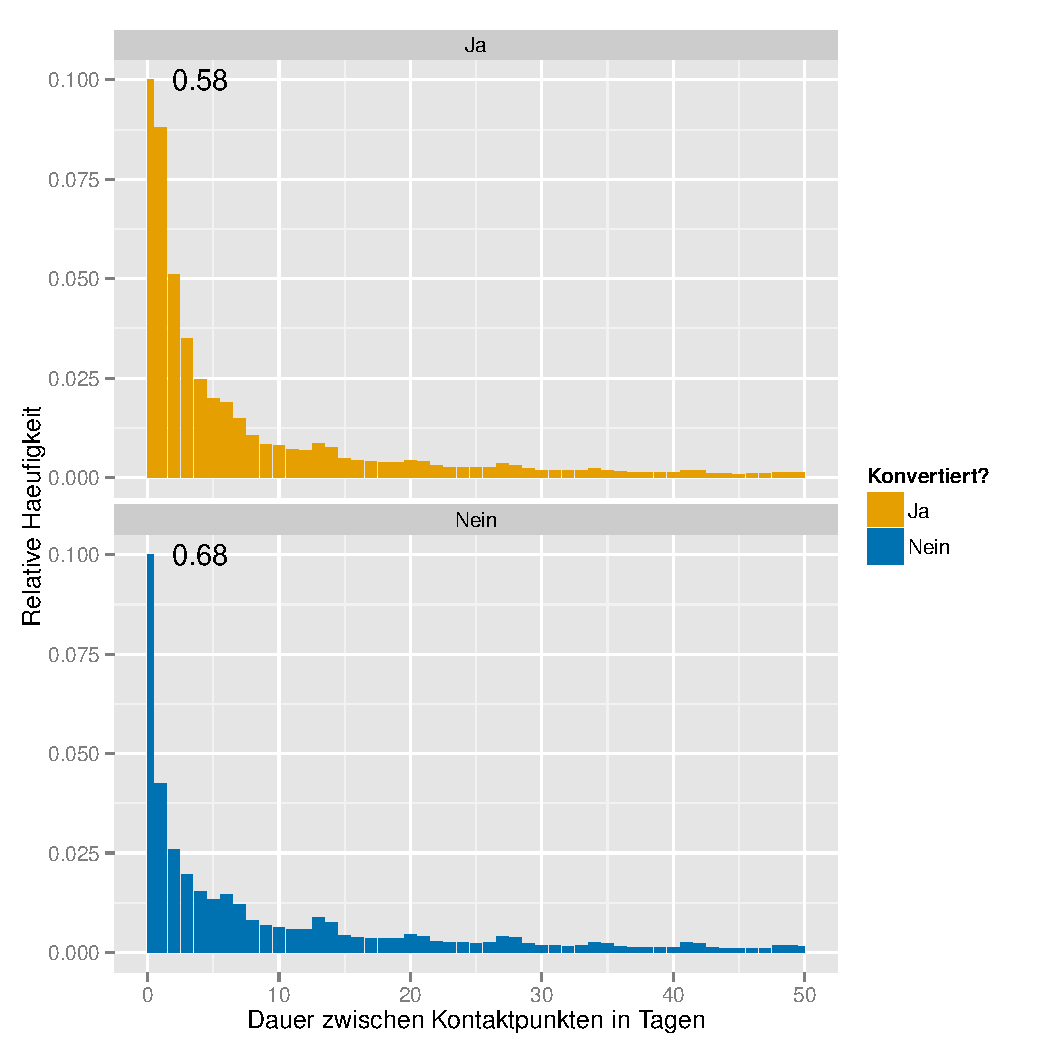
\includegraphics[scale=0.5]{timeSinceLast.pdf}
    \caption[Dauer zwischen zwei Kontaktpunkten]{Dauer zwischen zwei Kontaktpunkten in den konvertierten und nicht-konvertierten Funnels}
    \label{timeSinceLast}
\end{figure}

\subsubsection*{freq}
Die Frequenz wird wie folgt berechnet. Die Daten werden dahingehend gefiltert, dass für jeden Funnel nur der letzte Kontaktpunkt vorhanden ist. Die Variable \textit{timeSinceFirst} gibt somit wieder die Beobachtungsdauer des gesamten Funnels an. Daraufhin wird die Länge des Funnels (siehe Abbildung \ref{funnelLength}) durch die Beobachtungsdauer in Stunden geteilt, so dass eine Größe ensteht, die angibt, wieviel Kontaktpunkte der jeweilige Funnel pro Stunde hatte. Diese Frequenz wird in Abbildung \ref{freq} abgebildet, wobei auf der $x$-Achse die Länge der Funnels zwischen vier und $25$ aufgetragen ist. Für Funnels mit einem Kontaktpunkt existiert offentsichtlich keine Frequenz und die Längen zwei und drei werden nicht mit abgebildet, da die Frequenzen dort verhältnismäßig groß sind. Außerdem sind einige Boxplots nach oben hin abgeschnitten, da die Grenze der $y$-Achse auf $0.15$ gesetzt wurde, damit die Boxplots besser sichtbar sind, wobei der Median, das heißt der schwarze Balken in den Boxplots, für jeden Boxplot erkennbar bleibt. Die orangefarbigen Boxplots entsprechen den Frequenzen der konvertierten und die blauen den Frequenzen der nicht-konvertierten Funnels.\\
Für die Funnel Länge zwei liegt der Median der Frequenzen bei 1.22 in den konvertierten und bei 19.89 in den nicht-konvertierten Funnels sowie für die Länge drei bei 0.021 beziehungsweise 0.348.\\
Insgesamt ist zu erkennen, dass die Frequenzen in den nicht-konvertierten Funnels höher zu sein scheint. Das heißt in denjenigen Funnels die zu keiner Konvertierung führen liegen die Kontaktpunkte näher beieinander, während sie in den konvertierten Funnels mehr über die Zeit verteilt sind.\\
\begin{figure}[H]
		\centering
	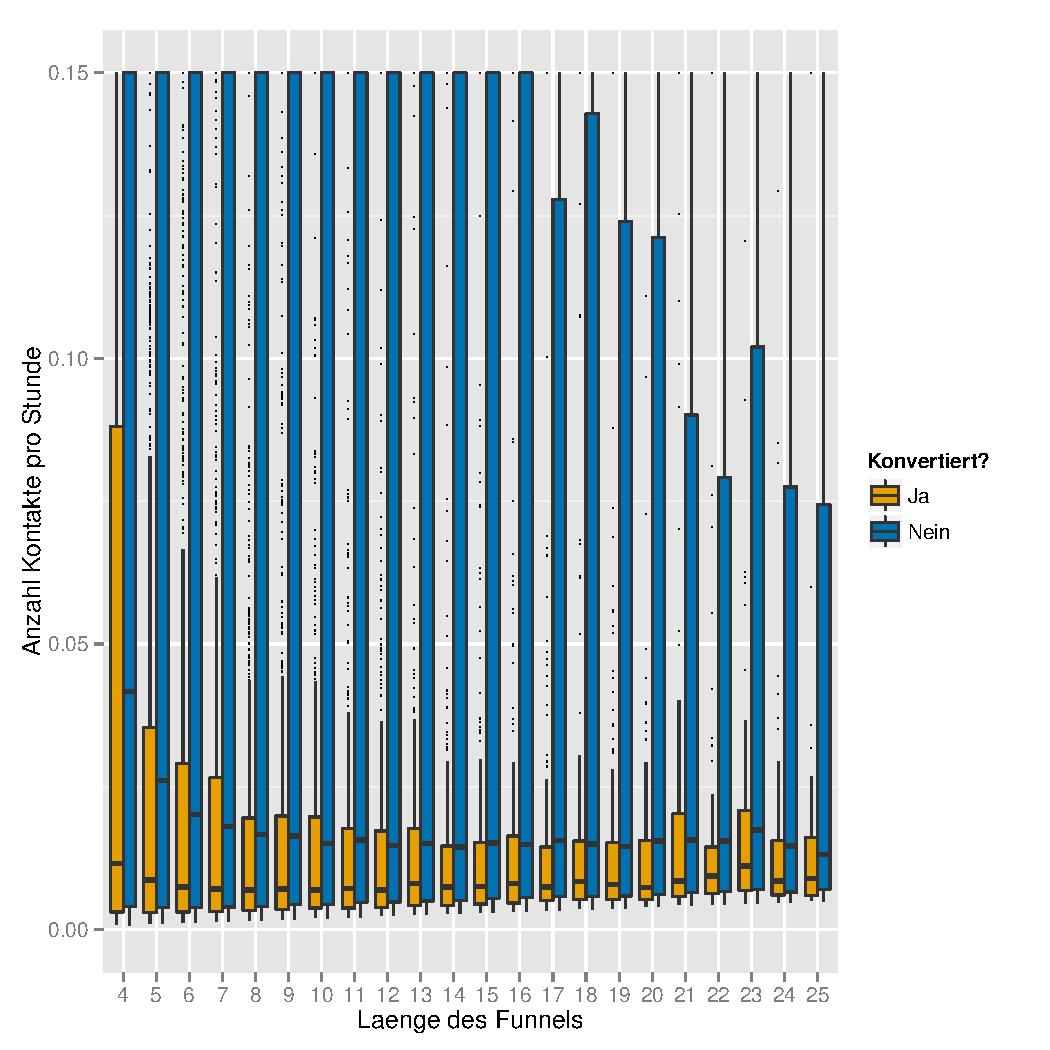
\includegraphics[scale=0.5]{freq.pdf}
	\caption[Frequenz der Kontaktpunkte]{Frequenz der Kontaktpunkte in konvertierten und nicht-konvertierten Funnels}
	\label{freq}
\end{figure}
